% !TEX root = ./rosbook_jp.tex
%-------------------------------------------------------------------------------
\chapterimage{chapter_head_8.pdf}

%-------------------------------------------------------------------------------
\chapter{センサによる情報の取得}\index{センサによる情報の取得}

7章で述べたように、ROSのアプリケーションソフトウェアはロボットパッケージとセンサパッケージに分けられる。本章ではこのセンサパッケージのうち、ロボットアプリケーション開発で多く用いられるUSBカメラ、レーザレンジファインダー(LRF)、デプスカメラに対し、必要なパッケージのインストール方法とパッケージの使用方法について、具体例を交えて解説する。

%-------------------------------------------------------------------------------
\section{USBカメラ}\index{USBカメラ}

カメラはロボットの眼であり、カメラによって得られる画像はロボット周囲の環境認識に極めて有効である。カメラ画像は、物体認識や顔認識、領域抽出や抽出された領域の追跡、複数台のカメラ(ステレオカメラ)を使った距離計測、地図生成、Visual-SLAM(カメラ画像を用いた位置と地図の同時推定)など、多くの用途に用いられる。
本節では、多種多様なカメラの中でも、特にUSBカメラを取り上げ、ROSでUSBカメラとPCを接続し、画像を表示する方法を実例を挙げて説明する。市販されている多くのUSBカメラは、USB video device class規格(UVC規格)を採用していることから、USBカメラは別名で「UVCカメラ」とも呼ばれる。UVC規格は2015年1月現在、バージョン1.5が最新である。UVC 1.5バージョンは、最新のUSB 3.0をサポートし、Linux、Windows、OS Xなど、ほぼすべてのオペレーティングシステムで使用できる。本書では、「UVCカメラ」よりも広く使用されている「USBカメラ」の名称を用いる。

%-------------------------------------------------------------------------------
\subsection{USBカメラ関連パッケージ}

ROSはUSBカメラに関連した様々なパッケージを提供している。詳細については、ROS Wiki(http://wiki.ros.org/Sensors/Cameras)で見ることができる。以下では、代表的なパッケージについて説明する。

\vspace{\baselineskip}
\noindent
\begin{description}
\item[libuvc-camera] UVC規格のUSBカメラを使用するためのインタフェースパッケージである。
\item[uvc-camera] USBカメラの設定を細かく変更できるインタフェースパッケージである。2台のカメラをつなげて、ステレオカメラとして利用することもできる。
\item[usb-cam] Bosch社が開発、公開したUSBカメラ用のインタフェースパッケージである。Bosch社が公開しているパッケージを使うときに必要な場合がある。
\item[freenect-camera、openni-camera、openni2-camera] KinectやXtionなど距離計測が可能なRGB-Dカメラのためのインタフェースパッケージである。これらのRGB-Dカメラにはカラーカメラも搭載されているが、カラーカメラだけを利用する場合にも、これらのパッケージが必要である。
\item[camera1394] IEEE 1394規格であるFireWireを使用するカメラ用のインタフェースパッケージである。
\item[prosilica-camera] 研究用に多く使用されているAVT社製prosilicaカメラ用のインタフェースパッケージである。
\item[pointgrey-camera-driver] 研究用に多く使用されているPoint Grey Research社製カメラ用のインタフェースパッケージである。
\item[camera-calibration] OpenCVのキャリブレーション機能を利用したカメラキャリブレーション関連パッケージである。ROSのカメラ関連のパッケージは、このパッケージを必要とすることが多い。
\end{description}

%-------------------------------------------------------------------------------
\subsection{USBカメラの使用方法}

本項では、USBカメラのパッケージの中でも最も広く利用されているuvc-camera\footnote{\url{http://wiki.ros.org/uvc\_camera}}を利用する。他のパッケージの使用方法もuvc-cameraと共通点が多いが、詳細についてはそれぞれのパッケージのWikiで確認してほしい。

\subsubsection{USBカメラの接続}

USBカメラを準備し、PCのUSBポートとUSBケーブルで接続する。

\subsubsection{カメラ情報の確認}

新しいターミナルウィンドウを開いて、lsusbコマンドにより接続が正しいことを確認する。UVC\footnote{\url{http://en.wikipedia.org/wiki/USB\_video\_device\_class}}規格のカメラであれば、以下の太文字のように、接続されたUSBカメラのメーカやUSB規格が表示される。この例では、Z-Star Microelectronics社のUSBカメラが認識されている。

\begin{lstlisting}[language=ROS]
$ lsusb
Bus 002 Device 004: ID 1a40:0101 Terminus Technology Inc. 4.Port HUB
Bus 002 Device 003: ID 048d:1336 Integrated Technology Express, Inc. SD/MMC Cardreader
Bus 002 Device 001: ID 1d6b:0002 Linux Foundation 2.0 root hub Bus 006 Device 001: ID 1d6b:0003 Linux Foundation 3.0 root hub
Bus 001 Device 009: ID 0ac8:3420 Z.Star Microelectronics Corp. Venus USB2.0 Camera
Bus 001 Device 008: ID 0a12:0001 Cambridge Silicon Radio, Ltd Bluetooth Dongle (HCI mode) Bus 001 Device 007: ID 046d:c52b Logitech, Inc. Unifying Receiver
Bus 001 Device 006: ID 1a40:0101 Terminus Technology Inc. 4.Port HUB Bus 001 Device 005: ID 0853:0134 Topre Corporation
Bus 001 Device 002: ID 8087:0024 Intel Corp. Integrated Rate Matching Hub Bus 001 Device 001: ID 1d6b:0002 Linux Foundation 2.0 root hub
Bus 002 Device 002: ID 8087:0024 Intel Corp. Integrated Rate Matching Hub
\end{lstlisting}

\subsubsection{ROS uvc-cameraカメラのパッケージのインストール}

ROSのUSBカメラドライバであるuvc-cameraパッケージをインストールする。

\begin{lstlisting}[language=ROS]
$ sudo apt-get install ros-indigo-uvc-camera
\end{lstlisting}

\subsubsection{ROS image関連パッケージのインストール}

画像処理と画像可視化のためのROS image関連パッケージをインストールする。

\begin{lstlisting}[language=ROS]
$ sudo apt-get install ros-indigo-image-*
$ sudo apt-get install ros-indigo-rqt-image-view
\end{lstlisting}

\subsubsection{uvc\_cameraノードの実行}

以下のようにuvc\_cameraノードを実行すると、「[WARN] [1423194481.257752159]: Camera calibration file /home/xxx/.ros/camera\_info/camera.yaml not found.」のように、カメラキャリブレーション\footnote{\url{http://wiki.ros.org/camera\_calibration}}に関連する警告が表示される。これは、キャリブレーションファイルが存在しないためであり、単に画像を表示するだけであれば無視しても構わない。キャリブレーション方法については、8.1.5項で詳しく説明する。

\begin{lstlisting}[language=ROS]
$ roscore
$ rosrun uvc_camera uvc_camera_node
\end{lstlisting}

\subsubsection{トピックスメッセージの確認}

以下のようにトピックメッセージを表示すると、カメラ情報(/camera\_info)と画像情報(/image\_raw)が配信されていることが確認できる。

\begin{lstlisting}[language=ROS]
$ rostopic list
/camera_info
/image_raw
/image_raw/compressed
/image_raw/compressed/parameter_descriptions /image_raw/compressed/parameter_updates
/image_raw/compressedDepth
/image_raw/compressedDepth/parameter_descriptions /image_raw/compressedDepth/parameter_updates
/image_raw/theora
/image_raw/theora/parameter_descriptions
/image_raw/theora/parameter_updates
/rosout
/rosout_agg
...
\end{lstlisting}

%-------------------------------------------------------------------------------
\subsection{画像情報の確認}

前項ではuvc\_camera\_nodeノードを実行し、画像情報が配信されていることを確認した。本項では、可視化ツールであるimage\_viewとrvizを利用して、画像を実際に表示してみる。もし以下の手順を実行しても画像が表示できない場合には、カメラのドライバや接続に問題がある。

\subsubsection{image\_viewノードによる確認}

まず、画像を表示するためにimage\_viewノードを実行しよう。つぎのコマンドで、「i\\mage:=/image\_raw」というオプションとともにimage\_viewノードを起動する。「image:=\\/image\_raw」は、上記のトピック一覧で確認した「/image\_raw」トピックを画像で表示するためのオプションである。

\begin{lstlisting}[language=ROS]
$ rosrun image_view image_view image:=/image_raw
\end{lstlisting}

図8-1のように、小さなウィンドウが現れ、カメラ画像が表示される。

\begin{figure}[htp]
  \centering
  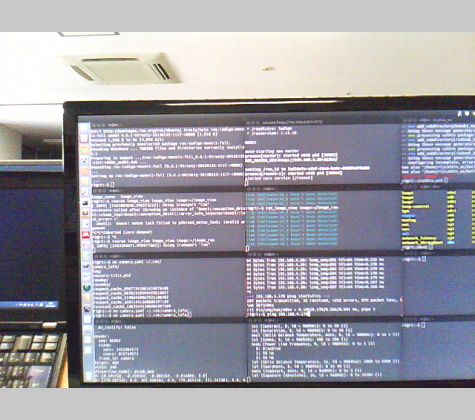
\includegraphics[width=10cm]{pictures/chapter8/pic_08_01.png}
  \caption{image\_viewノードを利用した画像表示}
\end{figure}


\subsubsection{rqt\_image\_viewノードによる確認}

次に5.2.4項で説明したrqt\_image\_viewを利用してみよう。rqt\_image\_viewはrqtプラグインとして、image\_viewにGUIを追加したものである。以下のようにrqt\_image\_viewノードを実行すると、図8-2に示すような画像が表示される。ただしimage\_viewとは異なり、GUI形式であり、上部のプルダウンメニューからトピックを選択することができる。

\begin{lstlisting}[language=ROS]
$ rqt_image_view image:=/image_raw
\end{lstlisting}

\begin{figure}[htp]
  \centering
  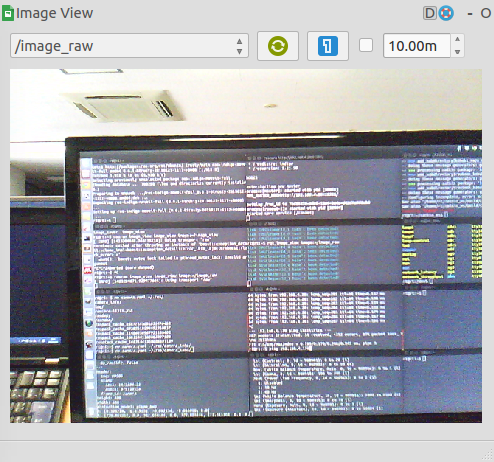
\includegraphics[width=10cm]{pictures/chapter8/pic_08_02.png}
  \caption{rqt\_image\_viewノードを利用した画像表示}
\end{figure}

\subsubsection{RVizによる確認}

最後に、可視化ツールであるRVizで確認してみる。RVizの詳細な説明は5.1節を参考にしてほしい。まず、次のコマンドでRVizを実行しよう。

\begin{lstlisting}[language=ROS]
$ rosrun rviz rviz
\end{lstlisting}

RVizが起動したら、Displaysオプションを変更する。RViz左下の<Add>をクリックして、図8-3のように[By display type]→[rviz]→[Image]を選択して画像表示を追加する。

\begin{figure}[htp]
  \centering
  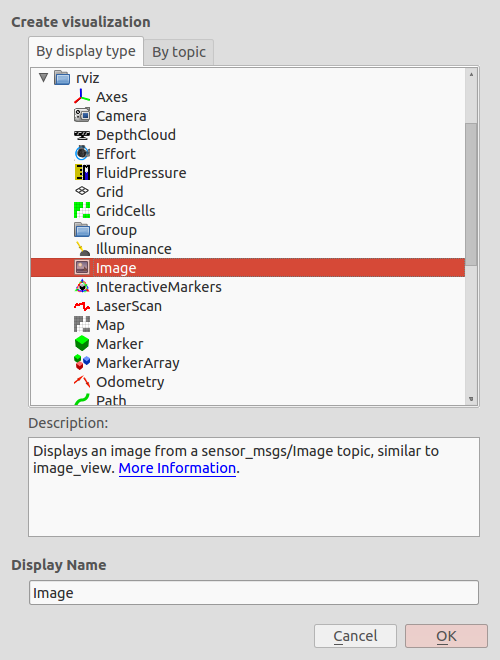
\includegraphics[width=10cm]{pictures/chapter8/pic_08_03.png}
  \caption{RVizに画像表示を追加}
\end{figure}

次に[Image]→[Image Topic]の値を「/image\_raw」に変更する。これにより、図8-4のように画像が表示される。

\begin{figure}[htp]
  \centering
  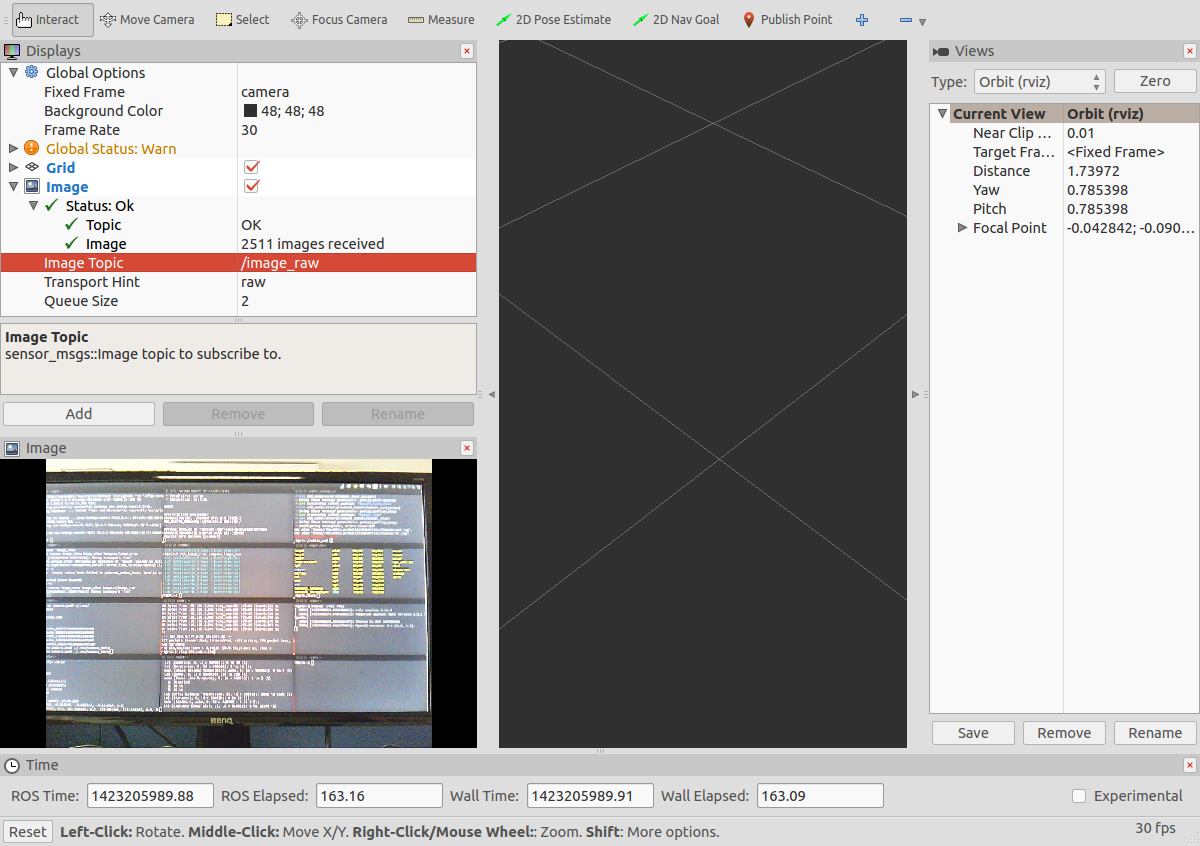
\includegraphics[width=10cm]{pictures/chapter8/pic_08_04.png}
  \caption{RVizを利用した画像表示}
\end{figure}

%-------------------------------------------------------------------------------
\subsection{リモート画像転送}

前項では、PCに直接USBカメラを接続して画像を表示した。本項では、ロボットのコンピュータ(マスター)に接続されたカメラの画像情報を、別のリモートコンピュータに表示する方法を説明する。

\subsubsection{カメラが接続されているコンピュータ上でマスターを起動}

マスターはどのコンピュータで起動しても構わないが、今回の例では、カメラが接続されているコンピュータをマスターとする。最初に行う設定はROS\_MASTER\_URIとROS\_HOSTNAMEなどのネットワーク変数の変更である。まず、geditなどの文書編集プログラムを使用して、次のように「.bashrc」ファイルを開く。

\begin{lstlisting}[language=ROS]
$ gedit ~/.bashrc
\end{lstlisting}

「.bashrc」ファイルを読み込み、一番下までスクロールして、次のようにROS\_MASTER\_URIとROS\_HOSTNAME変数を変更しよう。ただし、この例のIPアドレス(ROS\_MASTER\_URI、ROS\_HOSTNAME ともに192.168.4.100で、カメラが接続されたコンピュータのIPアドレス)は、あくまでも例であり、実際のPCのIPアドレスに変更する必要がある。 IPを確認するには、2.2.1項で説明したifconfigコマンドを使用する。

\begin{lstlisting}[language=bash]
export ROS_MASTER_URI = http://192.168.4.100:11311
export ROS_HOSTNAME = 192.168.4.100
\end{lstlisting}

次にroscoreコマンドでマスターを起動して、uvc\_camera\_nodeノードを実行する。

\begin{lstlisting}[language=ROS]
$ roscore
$ rosrun uvc_camera uvc_camera_node
\end{lstlisting}

\subsubsection{リモートコンピュータでの画像表示}

リモートコンピュータでも同様に、「.bashrc」ファイルを開いてROS\_MASTER\_URIとROS\_HOSTNAME変数を変更する。次のように、ROS\_MASTER\_URIはカメラが接続されたコンピュータのIPアドレス(192.168.4.100)とし、ROS\_HOSTNAME変数はリモートコンピュータのIPアドレス(ここでは192.168.4.120)に変更する。ここでもリモートコンピュータのIPアドレス192.168.4.120は一例なので、実際のコンピュータのIPアドレスをifconfigで確認し、正しく入力する必要がある。

\begin{lstlisting}[language=bash]
export ROS_MASTER_URI = http://192.168.4.100:11311
export ROS_HOSTNAME = 192.168.4.120
\end{lstlisting}

次にimage\_viewを起動する。

\begin{lstlisting}[language=ROS]
$ rosrun image_view image_view image:=/image_raw
\end{lstlisting}

以上により、リモートコンピュータにカメラ画像が表示されるはずである。本項は、ロボットに装着されたカメラの画像情報を、別のコンピュータで確認する方法を述べた。この方法を用いれば、ROSのネットワークを用いて遠隔地のロボットのカメラ画像を伝送し、確認できる。

%-------------------------------------------------------------------------------
\subsection{カメラキャリブレーション}

8.1.2項では、USBカメラを繋いでuvc\_cameraノードを実行すると、カメラのキャリブレーションに関連する警告が現れた。目的がカメラ画像の確認だけであれば、この警告は無視しても構わない。しかし、ステレオカメラによる距離測定や画像からレンズの歪みを除去したい場合には、警告に従ってカメラのキャリブレーションをおこなう必要がある。
カメラキャリブレーションとは、カメラ固有のパラメータを同定し、画像を補正する処理である。一般的に、複数台のカメラから得られた画像情報からカメラと対象物の間の正確な距離を計算するには、カメラの光学特性の情報が必要となる。特にレンズとイメージセンサとの距離(焦点距離)や画像中心座標、軸の傾き、レンズの歪み(収差)はカメラごとに異なり、それぞれのカメラで事前にキャリブレーションを行い、同定しておく必要がある。
ROSでは、OpenCVのカメラキャリブレーションを利用したキャリブレーションパッケージが提供されている。以下では、実際にUSBカメラをキャリブレーションする手順を示す。

\subsubsection{カメラキャリブレーションパッケージのインストール}

まず、以下のようにカメラのキャリブレーションパッケージをインストールして、uvc\_camera\_nodeノードを実行しよう。

\begin{lstlisting}[language=ROS]
$ sudo apt-get install ros-indigo-camera-calibration
$ rosrun uvc_camera uvc_camera_node set_camera_info:=/camera/set_camera_info
\end{lstlisting}

以下は、現在のカメラの情報を確認するコマンドである。このうち、D、K、R、Pがカメラキャリブレーションに関連するパラメータであり、ここでは初期値が表示されている。

\begin{lstlisting}[language=ROS]
$ rostopic echo /camera_info
header:
 seq: 690
 stamp:
  secs: 1423194537
  nsecs: 11617377
 frame_id: camera
height: 480
width: 640
distortion_model: ''
D: []
K: [0.0, 0.0, 0.0, 0.0, 0.0, 0.0, 0.0, 0.0, 0.0]
R: [0.0, 0.0, 0.0, 0.0, 0.0, 0.0, 0.0, 0.0, 0.0]
P: [0.0, 0.0, 0.0, 0.0, 0.0, 0.0, 0.0, 0.0, 0.0, 0.0, 0.0, 0.0]
binning_x: 0
binning_y: 0
roi:
 x_offset: 0
 y_offset: 0
height: 0
width: 0
do_rectify: False
---
\end{lstlisting}

\subsubsection{チェスボードの準備}

カメラキャリブレーションでは、図8-5のように黒と白の四角形からなるチェスボード(chess board)を使用する。以下のアドレスから、8 x 6のチェスボードの画像(横方向に8つの格子点、縦方向に6つの格子点)がダウンロードできる。

http://wiki.ros.org/camera\_calibration/Tutorials/MonocularCalibration?action=AttachFile&do=\\view&target=check-108.pdf

ダウンロードしたチェスボード画像をプリンタでA4サイズの紙に出力して、平らな板などに張り付けておく。このチェスボード画像は、位置や姿勢を変えながらカメラで複数回撮影し、キャリブレーション用の画像を作成するのに使われる。

\begin{figure}[htp]
  \centering
  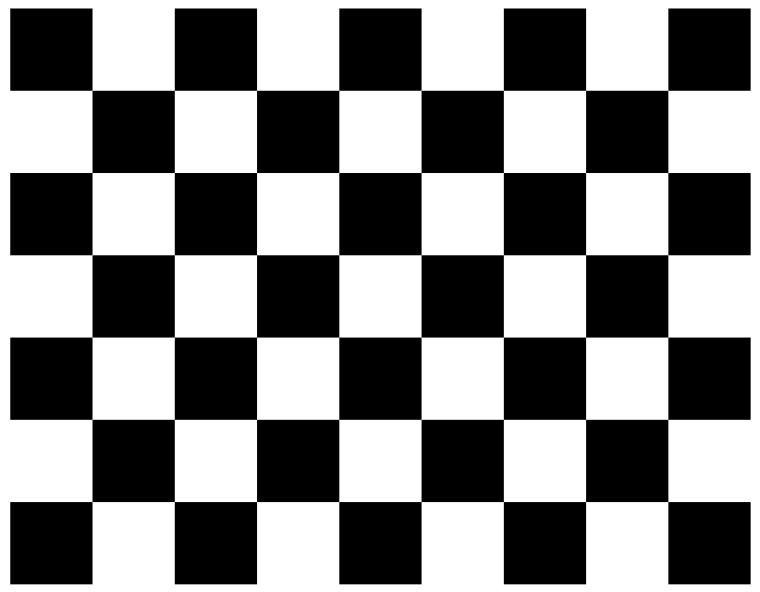
\includegraphics[width=12cm]{pictures/chapter8/pic_08_05.png}
  \caption{8 x 6チェスボード}
\end{figure}


\subsubsection{キャリブレーションの実行}

以下のコマンドで、カメラキャリブレーションを実行してみよう。キャリブレーションノードの引数「--size 8x6」はチェスボードの横x縦の格子点数、「--square 0.024」はチェスボードの四角形一つの実際のサイズ(単位はメートル)である。この四角形の大きさはプリンタによって異なる場合があるので、実際に印刷したチェスボードのサイズを定規で測って記入する。

\begin{lstlisting}[language=ROS]
$ rosrun camera_calibration cameracalibrator.py --size 8x6 --square 0.024 image:=/image_raw camera:=/camera
\end{lstlisting}

キャリブレーションのノードが実行されると、図8-6のようにGUI画面が現れる。チェスボードをカメラの前に置き、チェスボードを上下左右、斜め、あるいは回転させて、画像を複数回撮影しよう。撮影は、チェスボード全体が映っているときに自動で行われる。GUI画面の右側にX、Y、Size、Skewと表示されたバーがあるが、チェスボードを上下(Y)、左右(X)、前後(Size)、回転(Skew)させると、それぞれのバーの色が次第に緑に変化する。できるだけすべてのバーが緑色になるまで、チェスボードをいろいろな位置、角度に動かし続けよう。

\begin{figure}[htp]
  \centering
  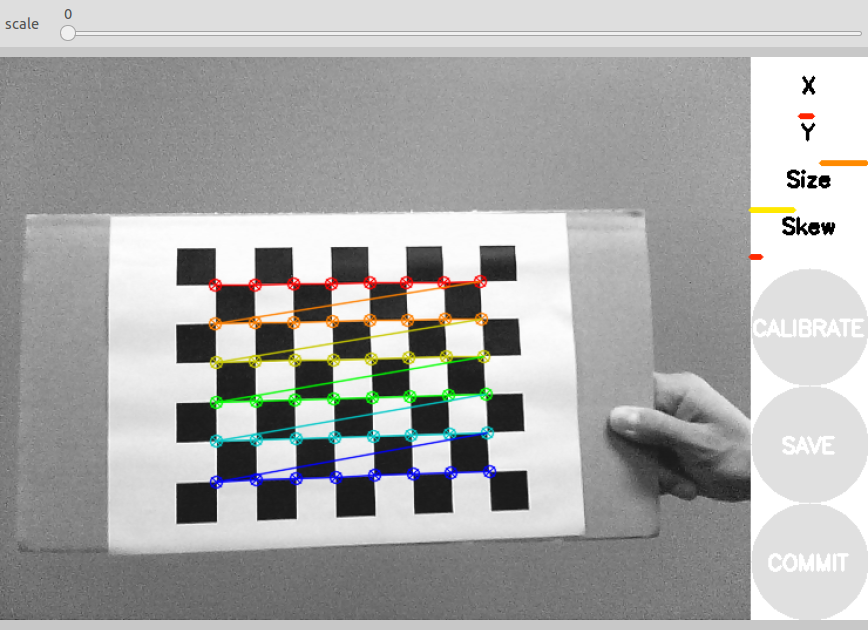
\includegraphics[width=12cm]{pictures/chapter8/pic_08_06.png}
  \caption{キャリブレーションGUIの初期状態}
\end{figure}

カメラでチェスボードを撮影すると、格子点検出などのキャリブレーションに必要な処理が自動的に行われる。図8-7は、チェスボード内部の格子点が検出された例である。

\begin{figure}[htp]
  \centering
  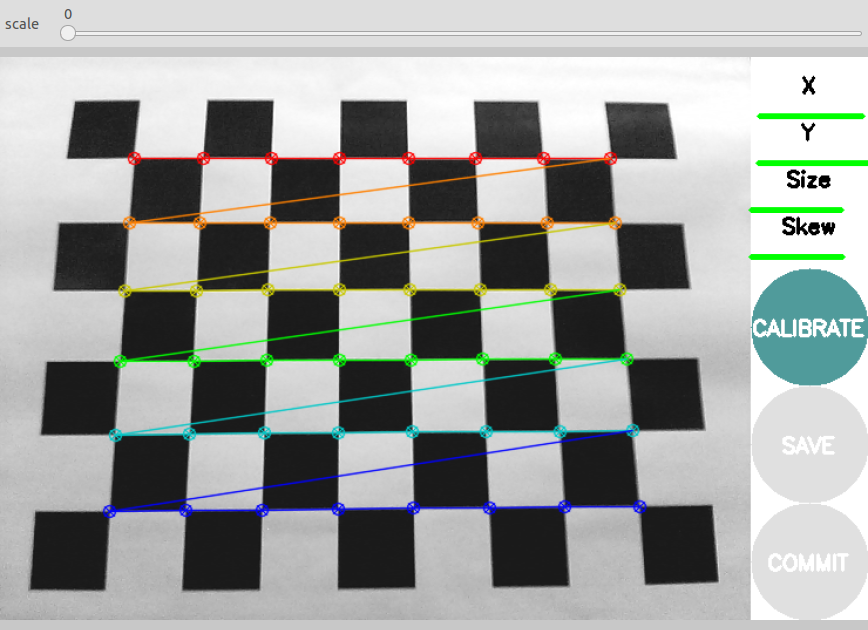
\includegraphics[width=12cm]{pictures/chapter8/pic_08_07.png}
  \caption{キャリブレーションGUI}
\end{figure}

十分な枚数の画像が自動的に撮影されると、キャリブレーション計算を実行するための<CALIBRATE>ボタンがアクティブになる。このボタンをクリックすると、キャリブレーション計算が実行される。キャリブレーション時間は約1〜5分程度である。計算が終了したら、<COMMIT>ボタンを押して、計算されたパラメータを保存する。<COMMIT>ボタンは、/camera/set\_camera\_infoサービスを呼び出し、求められたパラメータを「~/.ros/camera\_info/camera.yaml」ファイルに書き出す。以降、ROSで使用されるカメラ関連パッケージは、自動的にこのファイルを参照する。「~/.ros/camera\_info/camera.yaml」ファイルの例を以下に示す。なお、<SAVE>ボタンは、キャリブレーションで使用した画像やキャリブレーションデータをファイル(/tmp/calibrationdata.tar.gz)に保存する。

ファイル名: ~/.ros/camera\_info/camera.yaml
\begin{lstlisting}[language=ROS]
image_width: 640
image_height: 480
camera_name: camera
camera_matrix:
  rows: 3
  cols: 3
  data: [778.887262, 0, 302.058565, 0, 779.885146, 221.545303, 0, 0, 1]
distortion_model: plumb_bob
distortion_coefficients:
  rows: 1
  cols: 5
  data: [0.195718, -0.419555, -0.002234, -0.016098, 0]
rectification_matrix:
  rows: 3
  cols: 3
  data: [1, 0, 0, 0, 1, 0, 0, 0, 1]
projection_matrix:
  rows: 3
  cols: 4
  data: [794.464417, 0, 294.819501, 0, 0, 805.005371, 220.404173, 0, 0, 0, 1, 0]
\end{lstlisting}

このcamera.yamlには、カメラ内部行列camera\_matrix、歪み係数distortion\_coefficientsとステレオカメラのための補正行列rectification\_matrix、射影行列projection matrixなどが記録されている。それぞれの意味は「http://wiki.ros.org/image\_pipeline/CameraInfo」に詳しく説明されているので、そちらを参照されたい。
最後に、再びuvc\_camera\_nodeノードを実行する。今回はキャリブレーションファイルに関する警告が現れないことを確認しよう。

\begin{lstlisting}[language=ROS]
$ rosrun uvc_camera uvc_camera_node
[INFO] [1423200001.060824801]: using default calibration URL
[INFO] [1423200001.060926215]: camera calibration
URL: file:///home/xxx/.ros/camera_info/camera.yaml
\end{lstlisting}

さらに、「/camera\_info」トピックを確認すると、次のようにD、K、R、Pのパラメータが設定されたことが確認できる。

\begin{lstlisting}[language=ROS]
$ rostopic echo /camera_info
header:
seq: 98505
stamp:
secs: 1423204173
nsecs: 879739574
frame_id: camera
height: 480
width: 640
distortion_model: plumb_bob
D: [0.195718, -0.419555, -0.002234, -0.016098, 0.0]
K: [778.887262, 0.0, 302.058565, 0.0, 779.885146, 221.545303, 0.0, 0.0, 1.0]
R: [1.0, 0.0, 0.0, 0.0, 1.0, 0.0, 0.0, 0.0, 1.0]
P: [794.464417, 0.0, 294.819501, 0.0, 0.0, 805.005371, 220.404173, 0.0, 0.0, 0.0, 1.0, 0.0]
binning_x: 0
binning_y: 0
roi:
x_offset: 0
y_offset: 0
height: 0
width: 0
do_rectify: False
---
\end{lstlisting}

以上でカメラキャリブレーションは完了である。

%-------------------------------------------------------------------------------
\section{レーザレンジファインダー(LRF)}\index{レーザレンジファインダー(LRF)}

レーザレンジファインダー(Laser Range Finder, LRF)\footnote{\url{http://en.wikipedia.org/wiki/Laser_rangefinder}}はレーザを用いて物体との距離を計測するセンサであり、レーザスキャナ(Laser Scanner)、あるいはLIDAR(Laser Imaging Detection and Ranging)とも呼ばれる。
LRFは高速・高精度な距離計測が可能で、短時間で大量の点群データが取得でき、測定範囲も広い。これらの利点から、ロボット分野で最も頻繁に使用されているセンサの一つで、障害物検出やナビゲーション、SLAM(Simultaneous localization and mapping)\footnote{\url{http://en.wikipedia.org/wiki/Simultaneous_localization_and_mapping}}などで使われている。

ロボット分野で多く使用される代表的なLRFには、屋内外での無人走行車などに多く使用されているSICK\footnote{\url{http://www.sick.com/}}社のLMSシリーズ、室内ロボットに広く使用されている北陽電機のURGシリーズ\footnote{\url{https://www.hokuyo-aut.jp/products/}}、そして複数のレーザ光源を搭載した全方向レーザスキャナであるVelodyne社のHDLシリーズ\footnote{\url{http://velodynelidar.com/lidar/lidar.aspx}}などがある。これらのセンサはまだ高価格であり、一台当たり数十万~数百万円である。しかしRPLIDAR\footnote{\url{http://www.robopeak.com}}などの低価格LRFが販売され始めており、今後、一層の低価格化が期待される。
以降の項ではLRFの動作原理と必要なパッケージのインストール方法、利用方法について説明する。

\begin{figure}[htp]
  \centering
  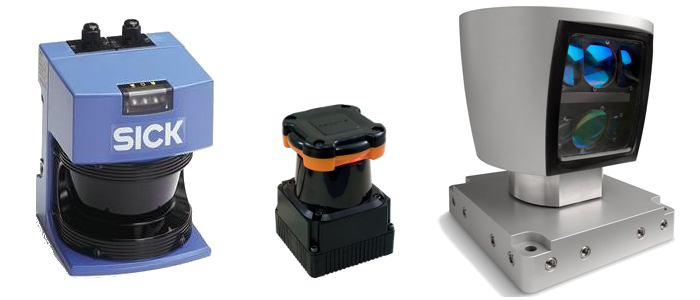
\includegraphics[width=12cm]{pictures/chapter8/pic_08_08.png}
  \caption{SICK LMS 210(左)、Hokuyo UTM-30LX(中央)、Velodyne HDL-64e(右)}
\end{figure}

%-------------------------------------------------------------------------------
\subsection{LRFによる空間計測}

LRFは、主に単一のレーザ光源(Velodyne HDLシリーズは複数)と反射鏡、そしてモーターで構成されている。LRFを起動すると、光源からレーザが投射され、モーターが内部の反射鏡を回転させてレーザを水平面に走査する。LRFは、走査されたレーザが物体表面で反射されて光源に戻るまでの時間から、物体までの距離を計測する。
図8-9の左図は、LRFが内部の反射鏡でレーザを走査している様子を表しており、LRFは図8-9の中図のようにLRFを中心に水平面内の物体までの距離を計測することができる。ただし、測定の原理上、図8-9の右図のように、計測物までの距離が遠いと計測点の間隔が広くなり、またノイズの影響も受け易くなる。

\begin{figure}[htp]
  \centering
  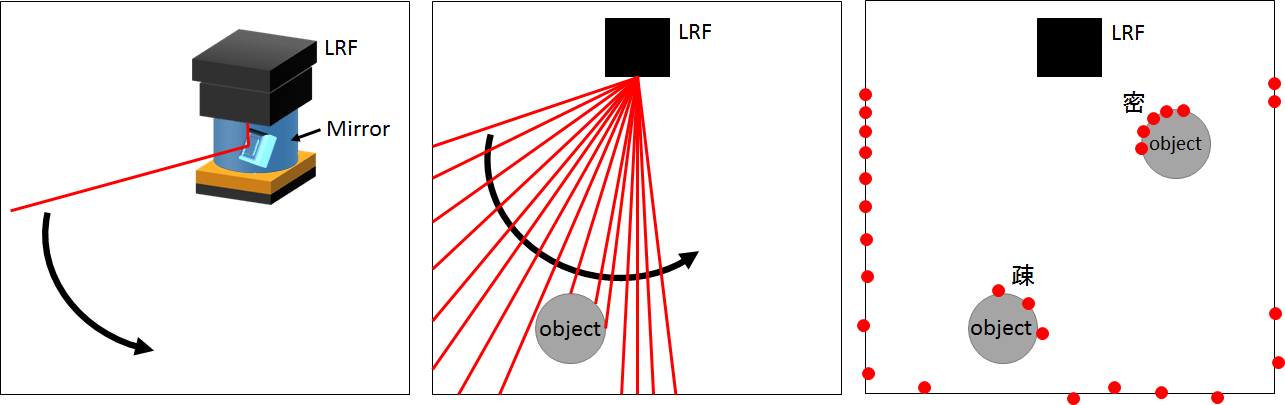
\includegraphics[width=\columnwidth]{pictures/chapter8/pic_08_09.png}
  \caption{LRFによる空間計測}
\end{figure}

LRFの使用にあたっては、以下の3つの点に留意する必要がある。
第一に、LRFが使用する出力の高いレーザは、眼の網膜を損傷する危険がある。レーザの安全基準\footnote{\url{https://ja.wikipedia.org/wiki/\%E3\%83\%AC\%E3\%83\%BC\%E3\%82\%B6\%E3\%83\%BC}}は出力や波長によってクラス1からクラス4まで複数のクラスに分けられ、クラスが高くなるほど危険性が増す。クラス1は、眼に対して安全な製品であり、直接裸目で見ても問題ない。詳しくは「レーザ製品の放射安全基準」(JIS C 6802)を参照してほしい。先に紹介したLRFは、すべてクラス1に該当する。
第二に、投射したレーザの反射光を捉えることで距離測定を行うため、レーザを反射しない対象物までの距離は計測できないことである。つまり、透明なガラス、ペットボトル、鏡、色の濃い物体などは、レーザが反射されずに透過したり、全反射したり、吸収されたり、複数の方向にレーザが拡散するため、距離値が得られない場合がある。
 第三に、一般には水平面を走査するセンサなので、水平面上の物体しか検出できない(Velodyne HDLシリーズは除く)。

%-------------------------------------------------------------------------------
\subsection{LRFの接続とテスト}

ROSでは、各社のLRFに対応する多くのパッケージが用意されている。例えば、SICK製LRFに対応したsicks300、sicktoolbox、sicktoolbox\_wrapperパッケージ、北陽電機製LRFのhokuyo\_node\footnote{\url{http://wiki.ros.org/hokuyo\_node}}、urg\_node\footnote{\url{http://wiki.ros.org/urg\_node}}パッケージ、Velodyne製HDLをサポートするVelodyneパッケージなどがある。本項では、ROSで北陽電機製UTM-30LX\footnote{\url{https://www.hokuyo-aut.jp/02sensor/07scanner/utm\_30lx.html}}を使用する例を挙げる。

\subsubsection{urg\_nodeパッケージのインストール}

まず最初に、以下のコマンドでurg\_nodeパッケージをインストールする。

\begin{lstlisting}[language=ROS]
$ sudo apt-get install ros-indigo-urg-node
\end{lstlisting}

なおROSのHydroバージョンより以前は、hokuyo\_nodeが使用されていたが、Hydroバージョン以降は新たなデバイスやイーサネット、マルチエコーに対応したurg\_nodeパッケージが使われるようになりつつある。

\subsubsection{LRF接続とアクセス権の変更}

北陽電機製UTM-30LXはインターフェースがUSB方式であり、PCとUSBケーブルで接続する。PCに接続されると、UTM-30LXは「ttyACMx」(xは数字)として認識される。例えば、以下ではUTM-30LXは「ttyACM0」として認識されている。

\begin{lstlisting}[language=ROS]
$ cd /dev
$ ls -l ttyACM*
crw-rw---- 1 root dialout 166, 0 Aug 11 14:30 ttyACM0
\end{lstlisting}

上の例では、ttyACM0のアクセス権が「crw-rw----」となっており、所有者(root、「r\\w-」)やグループ(dialout、「rw-」)以外にはアクセス権が与えられていない(「---」)ことが分かる。そこで、このインターフェースが誰でも利用できるように、chmodコマンドでアクセス許可を設定する。

\begin{lstlisting}[language=ROS]
$ sudo chmod a+rw /dev/ttyACM0
$ ls -l ttyACM*
crw-rw-rw- 1 root dialout 166, 0 Aug 11 14:35 ttyACM0
\end{lstlisting}

これより、アクセス権が「crw-rw-rw-」となり、所有者やグループ、その他のすべてにアクセス権が与えられたことが確認できる。

\subsubsection{urg\_nodeノードの実行}

では、urg\_nodeノードを実行し、LRFからデータを取得してみよう。まず、ターミナルウィンドウを開き、roscoreを実行する。

\begin{lstlisting}[language=ROS]
$ roscore
\end{lstlisting}

次にurg\_nodeノードを実行するため、別のターミナルウィンドウを開き、次のコマンドを実行する。

\begin{lstlisting}[language=ROS]
$ rosrun urg_node urg_node
\end{lstlisting}

\subsubsection{トピックメッセージの確認}

urg\_nodeノードを実行すると、「/scan」というトピックでLRFの計測値が送信される。次のコマンドでトピックの内容を確認できる。

\begin{lstlisting}[language=ROS]
$ rostopic echo /scan
  header:
    seq: 5866
    stamp:
      secs: 1407735556
      nsecs: 501421233
    frame_id: laser
angle_min: -2.35619449615
angle_max: 2.35619449615
angle_increment: 0.00436332309619
time_increment: 1.73611151695e.05
scan_time: 0.0250000003725
range_min: 0.0230000000447
range_max: 60.0
ranges: [0.9929999709129333,1.3346457658567, .............................
\end{lstlisting}

これより、frame\_idはlaserに設定されており、走査角度は最小-135°(-2.35619449615\\ラジアン)から最大135°までの270°である。また、角度分解能(angle\_increment)は0.25°(0.00436332309619 ラジアン)であり、1スキャン270°あたり1,080回の距離計測が行われ、1スキャンにかかる時間(scan\_time)は25msecであることなども確認できる。

%-------------------------------------------------------------------------------
\subsection{LRFの距離情報の確認(RViz)}

次に、RVizを用いてLRFの距離情報を確認する。まずRVizを実行して、次の手順で表示オプションを変更する。

\begin{itemize}
\item 設定の[Global Options]→[Fixed Frame]を「laser」に変更する。
\item RViz左下の<Add>ボタンをクリックした後、[Axes]を選択して軸を追加する。軸の形状は図8-10のように詳細設定で変更できる(LengthとRadius)。
\item RViz左下の<Add>ボタンをクリックした後、[LaserScan]を選択して追加する。図8-10のように詳細設定でトピックや色を変えることができる(TopicとColor Transformer、Color)。
\end{itemize}

\begin{figure}[htp]
  \centering
  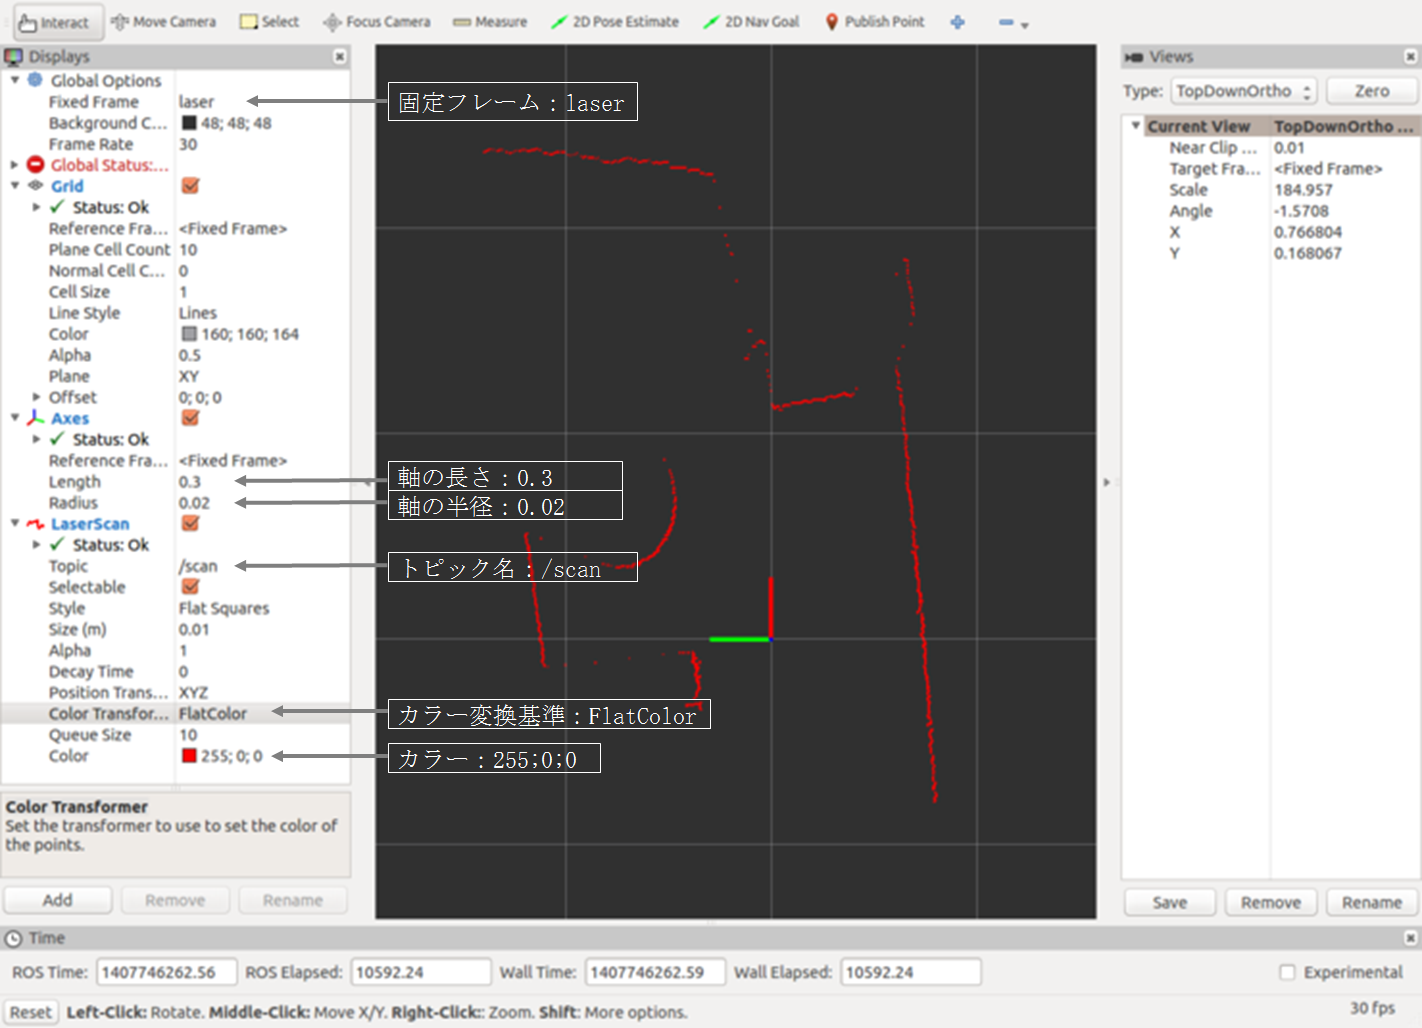
\includegraphics[width=\columnwidth]{pictures/chapter8/pic_08_10.png}
  \caption{RVizによるLaserScanの表示}
\end{figure}

図8-10のように周辺の物体の輪郭が表示される。灰色の格子の間隔が1mに設定されており、実際の大きさを知ることができる。

%-------------------------------------------------------------------------------
\subsection{LRFの用途}

LRFは様々な用途に用いられるが、代表的な例としてSLAM(Simultaneous Localization And Mapping)がある。SLAMとは、図8-11のように、ロボットにLRFなどの外界センサを取り付け、ロボットの自己位置同定と周辺の地図作成を同時に行う手法である。SLAMについては10章で詳しく説明する。

\begin{figure}[htp]
  \centering
  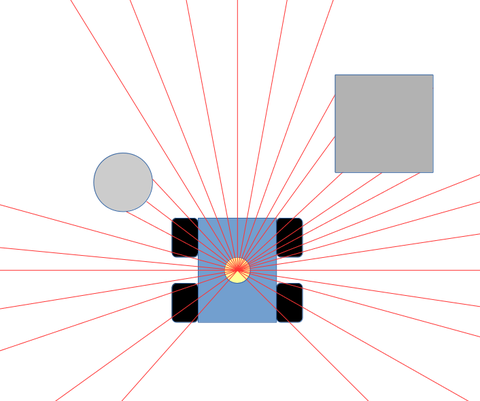
\includegraphics[width=12cm]{pictures/chapter8/pic_08_11.png}
  \caption{LRF活用例1: 移動ロボットの障害物検出}
\end{figure}

また、LRFを床面上に設置して固定することで、図8-12のようにLRF周囲にある様々な物体の位置や、検出された足の動きから人の位置を検出、追跡することもできる。

\begin{figure}[htp]
  \centering
  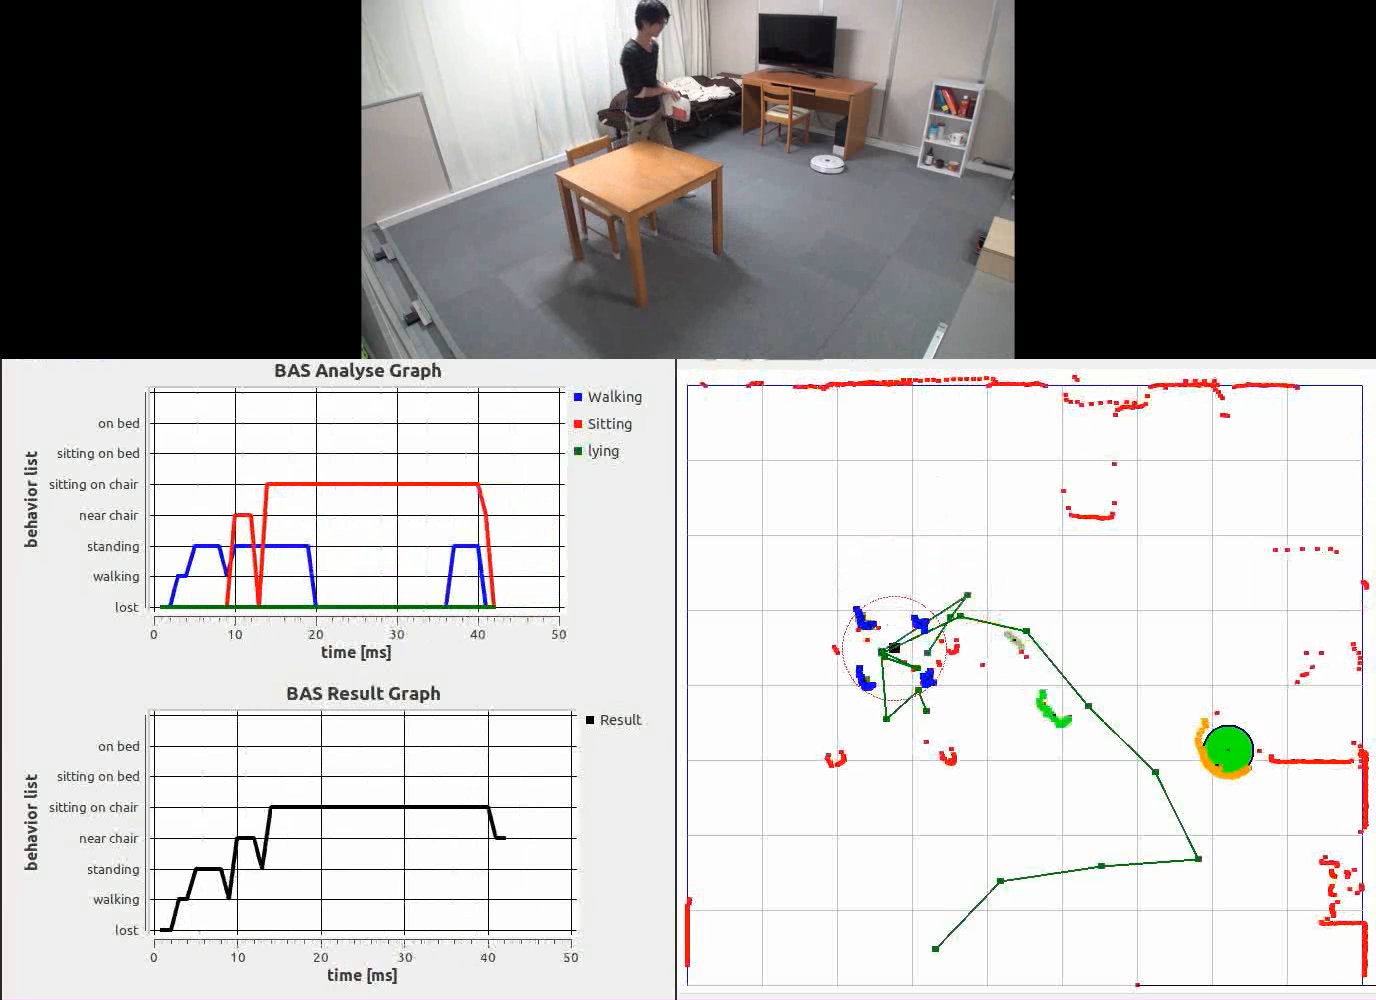
\includegraphics[width=12cm]{pictures/chapter8/pic_08_12.png}
  \caption{LRF活用例2: 人と物体の検出(動画はhttps://youtu.be/2cATgSHOVtcを参照)}
\end{figure}

%-------------------------------------------------------------------------------
\section{デプスカメラ}\index{デプスカメラ}

デプスカメラは 2次元ので距離(距離画像)が一度に得られるセンサであり、深度センサ、あるいはデプスセンサとも呼ばれる。カラー映像が同時に取得できる場合にはRGB-Dカメラとも呼ばれるが、本書ではすべてデプスカメラと呼ぶことにする。
デプスカメラの距離測定の方式として、様々なものが提案されている。ここでは、なかでも代表的なToF方式(Time of Flight)\footnote{\url{http://en.wikipedia.org/wiki/Time\_of\_flight}}とパターン投影方式(Pattern projection)を紹介する。

\subsubsection{ ToF方式}

ToF方式は近赤外光などを投射し、対象物表面で反射して戻るまでの時間(Time of Flight)から距離を測定する。一般的には光投射部と受光部が対になり、ピクセルごとに距離を読み取る。ToF方式のデプスカメラは構造が複雑なため、次に説明するパターン投影方式のカメラよりも一般に高価である(近年では、位相差や高速シャッターを利用した、低価格なToF方式のセンサも開発されている)。
ToF方式のセンサ\footnote{\url{http://en.wikipedia.org/wiki/Time-of-flight\_camera}}としては、パナソニックのD-IMager、MESA Imaging社SwissRanger、Fotonic社FOTONIC-B70、pmdtechnologies社CamCubeとCamBoard、SoftKinectic社DepthSense DSシリーズ、Microsoft社から最近発売されたKinect 2などがある。

\begin{figure}[htp]
  \centering
  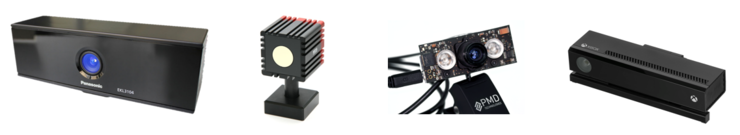
\includegraphics[width=12cm]{pictures/chapter8/pic_08_13.png}
  \caption{左からD-IMager、SwissRanger、CamBoard、Kinect2}
\end{figure}

\subsubsection{パターン投影方式}

パターン投影方式を使用しているデプスカメラには、Microsoft社のKinect\footnote{\url{http://en.wikipedia.org/wiki/Kinect}}やASUS\\社のXtion\footnote{\url{http://www.asus.com/Multimedia/Xtion\_PRO\_LIVE/}}、PrimeSense社のCarmine、Capriなどがあり、最近ではOccipital社からStructure Sensor\footnote{\url{http://structure.io/}}が発売されている。これらのデプスカメラは、共通してPrimeSen\\se社のPrimeSense SoC(System on a Chip、半導体チップ上に機能を集積した集積回路)を使用している。

\begin{figure}[htp]
  \centering
  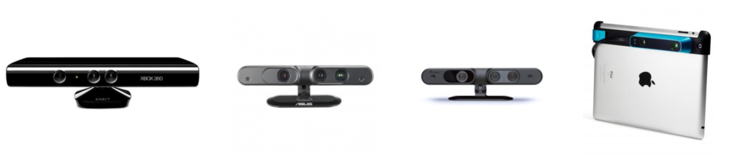
\includegraphics[width=\columnwidth]{pictures/chapter8/pic_08_14.png}
  \caption{左からKinect Xbox、Xtion、Carmine、Structure Sensor}
\end{figure}

PrimeSense社のPrimeSense SoCを使用したデプスカメラは、一対の赤外線プロジェクターと赤外線カメラからなるセンサで、特殊な投影パターンを持つ赤外線ドットを計測物体に投影し、この点の分布を赤外線カメラで計測している。ここで計測物体上の赤外線ドットのパターンは、平らな物体であれば投影パターンと同じであるが、障害物の形状が変化すると歪みが生じる。図8-16は壁を計測したときに赤外線ドットのパターンである。ドットパターンの変形量と赤外線プロジェクター・赤外線カメラ間の距離を用いると、物体表面の各点までの距離が計算できる。

\begin{figure}[htp]
  \centering
  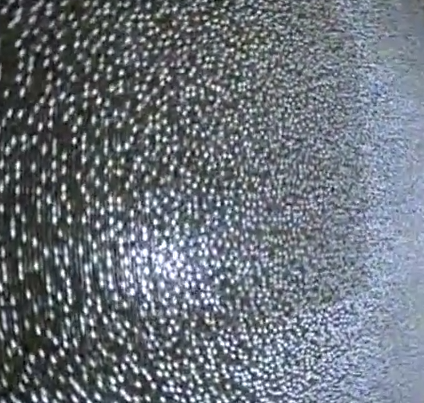
\includegraphics[width=\columnwidth]{pictures/chapter8/pic_08_15.png}
  \caption{Kinectのドットパターンの例}
\end{figure}


この方式を採用したデプスカメラは、低価格であり、また高速で高精度の距離画像が取得できることなどから注目を集めた。その後、PrimeSense社が自社のPrimeSense SoCを搭載したデプスカメラCarmine、Capriを発表した。また、同じSoCチップを搭載したMicrosoft社のKinectは、卓上ゲーム機Xboxのコントローラとして市販され、広く普及した。その後も、PCでの使用に特化したAsusのXtionなどが発売された。
しかし、2013年12月にApple社がPrimeSense社を買収し、PrimeSense社のCarmine、Capri製品やMicrosoft社のKinect、Asus社のXtionが販売中止となった。PrimeSense SoCを搭載した最後の製品であるOccipital社のStructure Sensorは、現在も販売を継続しているかが、今後も安定した供給が可能かは不明である。
現在は、GoogleのTangoプロジェクトやPrimeSense社買収後のApple社の製品、ToF系のCanesta社を買収したMicrosoft社のKinect 2などに関心が集まっている。

%-------------------------------------------------------------------------------
\subsection{OpenNI}

OpenNI(Open Natural Interaction)\footnote{\url{http://en.wikipedia.org/wiki/OpenNI}}は、PrimeSense社を中心にWillow Garage社、ASUS社が協力して開発された、PrimeSense SoC搭載製品のドライバやさまざまなAPIライブラリをまとめたソフトウエア群である。ここでNI(Natural Interaction)とは、人間と機械との自然なコミュニケーションを意味し、キーボードやマウスではなく、全身動作や手足の動きなどの人間の自然な動作を介した直感的なコミュニケーションの実現を目指している。
OpenNIには、距離画像やそれから得られる点群データだけでなく、スケルトン(骨格)の抽出やジェスチャー認識を行うミドルウェアであるNITEなども含まれている。OpenNIは、PrimeSense社がApple社に買収された後、一時的に開発中止となったが、現在ではOccipital社がGithubリポジトリ\footnote{\url{https://github.com/occipital/openni2}}を公開し、開発を続けている。またOpenNI以外にも、Microsoft社のKinect for Windows SDKの発表直後に、Kinectを初めてハッキングし、無償で公開されたことで有名なlibfreenectがある。

%-------------------------------------------------------------------------------
\subsection{PCL (Point Cloud Library)を用いた点群処理}

デプスセンサから得られた各画素の距離値と方向から、3次元空間上の一点の座標を得ることができる。この点を画像全体で計算すると、点の集合である点群(Point Cloud)が得られる。ROSでは、この点群処理にPCL(Point Cloud Library)\footnote{\url{http://pointclouds.org/}}と呼ばれるライブラリが利用できる。
PCLは、PCD(Point Cloud Data)形式の点群データに対し、フィルタリング、セグメンテーション、特徴抽出、モデルフィッティングなどの様々な処理を提供するライブラリである。

PCLをROSで使用するには、まず以下のようにlibpclパッケージをインストールする必要がある。

\begin{lstlisting}[language=ROS]
$ sudo add-apt-repository ppa:v-launchpad-jochen-sprickerhof-de/pcl
$ sudo apt-get update
$ sudo apt-get install libpcl-all
\end{lstlisting}

また、PCLをROSで使用する際に便利なpcl\_rosパッケージもインストールしておく。

\begin{lstlisting}[language=ROS]
$ sudo apt-get install ros-indigo-pcl-ros
\end{lstlisting}

では、PCLの標準の点群ファイル形式であるPCDファイルを読み込み、RVizで表示してみよう。まずRVizを実行して、次の手順で表示オプションを変更する。

\begin{itemize}
\item 設定の[Global Options]→[Fixed Frame]を「map」に変更する。
\item RViz左下の<Add>ボタンをクリックした後、[PointClound2]を選択して点群表示を追加する。
\item 新しいターミナルウィンドウを開き、pcl\_rosパッケージのpcd\_to\_pointcloudノードを実行する。ただしここでは、点群ファイル名はcloud\_file.pcdとする。
\end{itemize}

\begin{lstlisting}[language=ROS]
$ rosrun pcl_ros pcd_to_pointcloud cloud_file.pcd _frame_id:=/map
\end{lstlisting}

これにより、図8-17 のようにRVizに点群データが表示される。

\begin{figure}[htp]
  \centering
  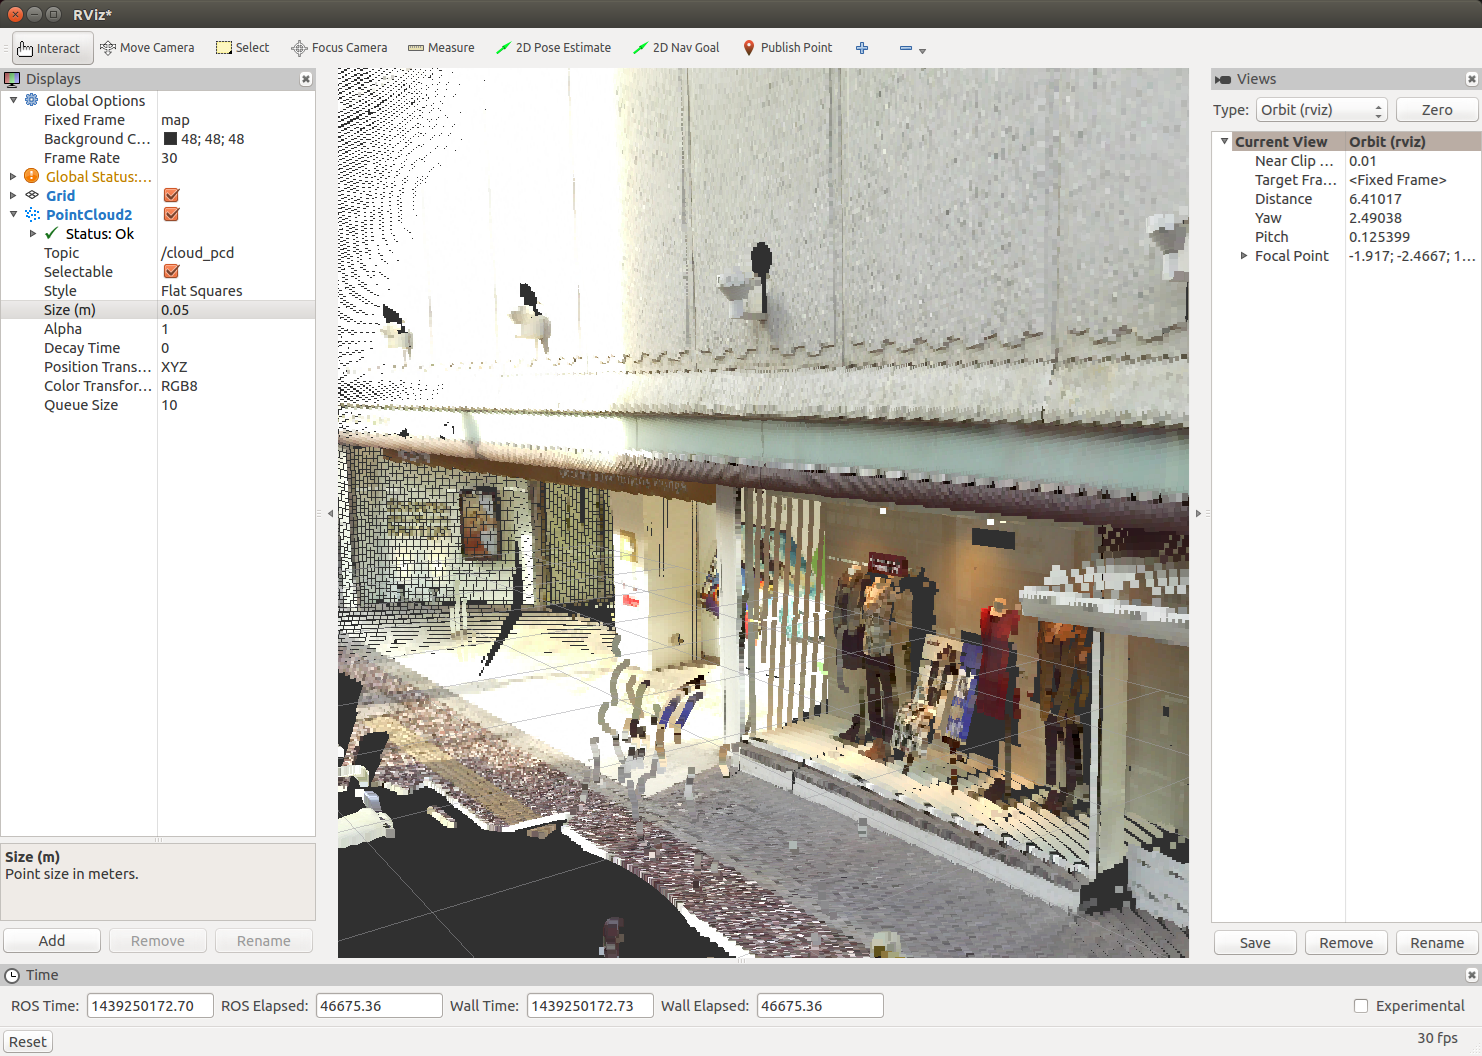
\includegraphics[width=\columnwidth]{pictures/chapter8/pic_08_16.png}
  \caption{RVizによるPCD点群データの表示}
\end{figure}

%-------------------------------------------------------------------------------
\subsection{デプスカメラのドライバのインストールと起動}

本項では、ASUS社Xtionを使用し、ROSを用いて画像の取得から表示までを行う。以下の手順に従って、デプスカメラのドライバをインストールして起動する。

\begin{itemize}
\item ROSのOpenNI関連パッケージをダウンロードしてインストールする。
\end{itemize}

\begin{lstlisting}[language=ROS]
$ sudo apt-get install ros-indigo-openni2-camera ros-indigo-openni2-launch
\end{lstlisting}

\begin{itemize}
\item Xtion用ドライバをインストールする。Xtionの購入時に同梱されているCDにXtio\\n用ドライバが含まれているので、それをインストールする。
\end{itemize}

\begin{lstlisting}[language=ROS]
$ tar -xvf Sensor-Bin-Linux-x64-v5.1.0.41.tar.bz2
$ cd Sensor-Bin-Linux-x64-v5.1.0.41/
$ sudo sh install.sh
\end{lstlisting}

\begin{itemize}
\item openni2\_launchパッケージのopenni2.launchファイルを実行する。
\end{itemize}

\begin{lstlisting}[language=ROS]
$ roscore
$ roslaunch openni2_launch openni2.launch
\end{lstlisting}

%-------------------------------------------------------------------------------
\subsection{点群情報の確認}

次に、RVizを用いて点群データを表示する。RVizを実行して、次の手順で表示オプションを変更する。

\begin{itemize}
\item 設定の[Global Options]→[Fixed Frame]を「camera\_depth\_frame」に変更する。
\item RViz左下の<Add>ボタンをクリックして、[PointCloud2]を選択して追加する。その後、図8-18に示すように「Topic」を「/camera/depth/points」、点群の模様である「Style」を「FlatSquares」、点群のサイズである「Size」を「0.01」に設定を変更する。
\item 図8-18のように点群データを確認することができる。色の基準をX軸に指定したので、点群がX軸から遠ざかるほど紫色に表示される。
\end{itemize}

\begin{figure}[htp]
  \centering
  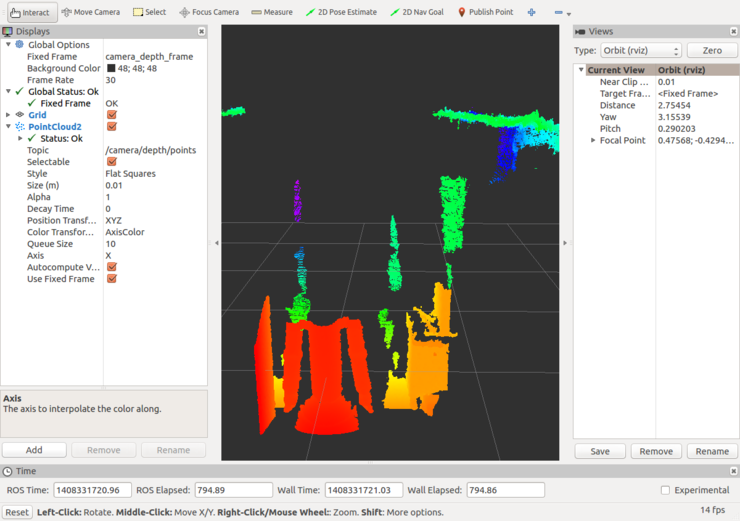
\includegraphics[width=10cm]{pictures/chapter8/pic_08_17.png}
  \caption{RVizによる点群表示}
\end{figure}

%-------------------------------------------------------------------------------
\subsection{デプスカメラの用途}

デプスカメラの用途は多岐に渡るが、代表的な例に3次元SLAMや、移動ロボットや無人自動車などで用いられる障害物回避、あるいは人の骨格情報などを利用したヒューマンインタフェースなどがある。例えば、図8-17の二次元バーコードを読み取り、デプスカメラを用いたモーションキャプチャやロボットの遠隔操作、ジェスチャーを使用した移動ロボットへの指示などを紹介する動画を参照されたい。

\begin{figure}[htp]
  \centering
  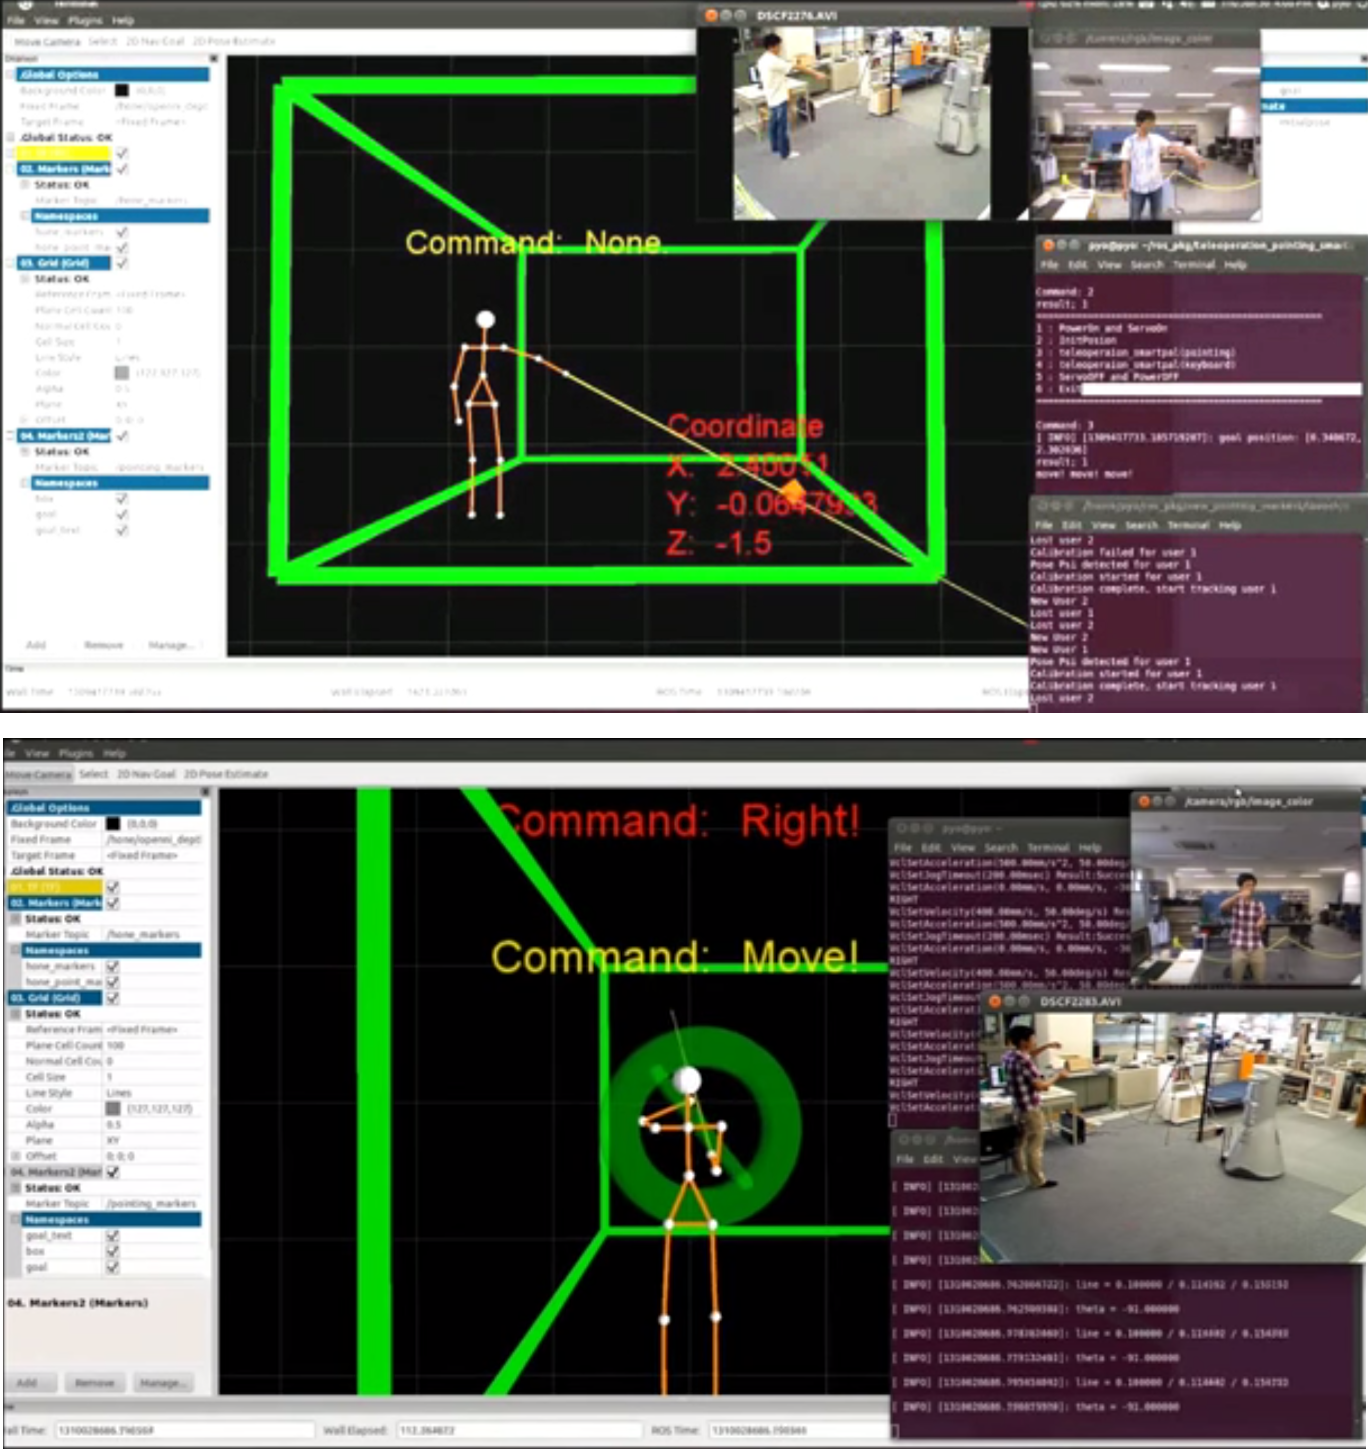
\includegraphics[width=10cm]{pictures/chapter8/pic_08_18.png}
  \caption{デプスカメラの用途の例}
\end{figure}

%-------------------------------------------------------------------------------
